\chapter{Architecture of \lpas{}}
\label{chap:num_4}

The following chapter provides the overview of the architecture of \lpas. Explains the main components of the Storage as well as how it is being integrated into LinkedPipes Applications platform.

\section{High level overview}

While the majority of components were described in detail in \ref{chap:num_1}, the overview architecture provided in this section shows more specific details on how all the external and internal components of the system are interacting. One of the essential details represented in the figure \ref{fig:lpas_high_level_architecture} is the separation between codebases of \lpa{} and \lpas{}. The \lpa{} Frontend is imports the \lpas{} as an npm package and performs all interactions with Solid using the provided functionality of the package. In some sense, \lpas{} is being threated as an additional rudimentary backend and database layer on top of existing internal components inside \lpa{}. This is due to several functional requirements that \lpas{} package implements,  such as \textit{user authentication}, \textit{storage crud operations} and etc.

\begin{figure}[h]
\centering
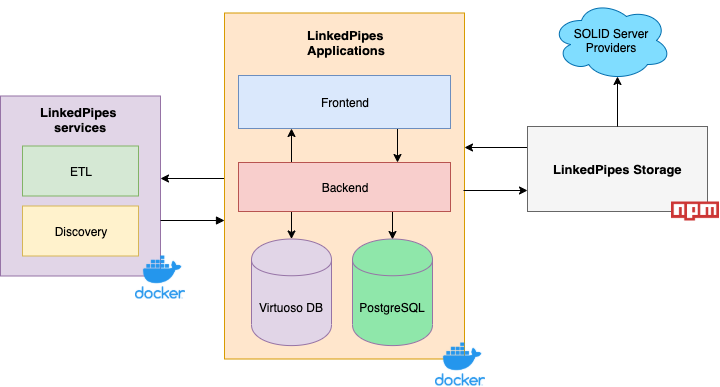
\includegraphics[width=14cm]{lpas_high_level_architecture.png}
\caption{High level overview of \lpa{} and \lpas{} interactions}
\label{fig:lps_authentication_sequence_diagram.png}
\end{figure}

As additionally demonstrated, the figure \ref{fig:lpas_high_level_architecture} also has Docker icons displayed under some modules. This is to indicate where the production-ready service is hosted. For instance, in the case of the \lpas{}, the end goal is the npm registry, while \lps{} and \lpa{} are all hosted in the docker registry where each internal component is a docker container.
The generic interaction flow usually involves direct communication between the \lpa{} frontend and \lpas{} package. The internal frontend component have various React components implemented using the \lpas{} package that provide navigation and interaction with \solid{} Pods. While the package is designed under the assumption that the \lpa{} is the only user of the package, some abstractions are generic enough and have the potential to be used outside of the scope of the main functional requirements. 

\section{The Storage}

The initial architecture and implementation draft of \lpas{} were different from what is presented in this chapter.  \solid{} related logic was firstly a part of the \lpa{} codebase. Therefore, significantly complicating unit testing and defining the difference the code implemented within the scope of the \lpa{} and \lpas{} projects. Later on, a decision was made to separate the logic of the \lpas{} and move it in the separate codebase. The majority of abstractions that were initially designed to be inside the \lpa{} codebase, consisted of various wrappers and crud functions to interact with \solid{} servers. Their design was refined and aggregated into specific abstractions, each responsible for covering the functional requirements from \lpa{} project.

\begin{figure}[h]
\centering
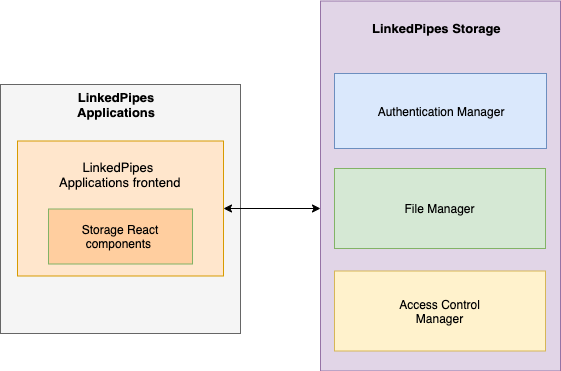
\includegraphics[width=14cm]{lpas_high_level_abstractions.png}
\caption{Main abstractions of \lpas.}
\label{fig:lpas_high_level_architecture}
\end{figure}

Let us start by describing the main abstractions providing the functionality of \lpas{}.

\subsection{Authentication Manager}

The Authentication Manger is responsible for wrapping \solid{} \textit{WebID} based authentication logic into a simple and developer friendly abstraction. As already mentioned in chapter \ref{chap:num_3}, the usage of \textit{WebID} protocols is one of many benefits of \solid{}, in contrast with popular authentication protocols used in centralized silos, it is completely agnostic to specific authentication mechanisms, allowing our single abstraction to support any arbitrary \textit{WebID-OIDC} compliant \solid{} provider.

At the moment of writing this, the official \solid{} specification states to support the following protocols:
\begin{itemize}
\item WebID-TLS  - is one of the primary authentication protocols that relies on WebIDs instead of usernames. The passwords are replaced with certain cryptographic certificates as bearer tokens and is stored within user's browser.
\item WebID-OIDC - alternative authentication protocol based on OAuth2 and OpenID Connect protocols and adjusted to support the concept of WebID. This is in fact the primary authentication option provided by \lpas{}, later chapters will provide reasoning behind why this ended up being more intuitive option to cover the authentication requirement for \lpa{}.   
\end{itemize}

\subsubsection{Interacting with frontend}

Sequence diagram on figure \ref{fig:lps_authentication_sequence_diagram} demonstrate an example on how the Authentication Manager will be used within the \lpa{} Frontend and how it will interact with \solid{} Providers.


\begin{figure}[h]
\centering
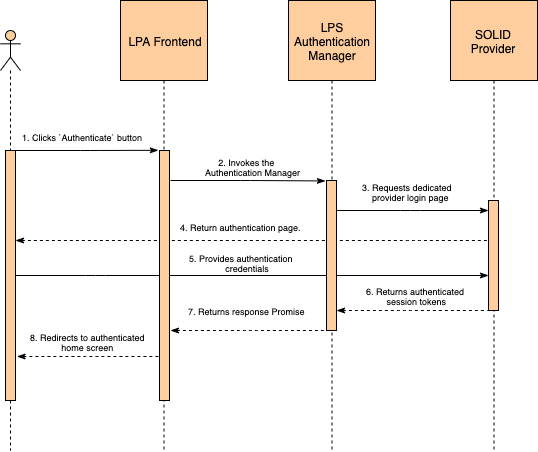
\includegraphics[width=14cm]{lps_authentication_sequence_diagram.png}
\caption{Sequence diagram for \textit{authenticate} operation invoked from \lpa{} frontend.}
\label{fig:lps_authentication_sequence_diagram}
\end{figure}

\subsection{File Manager}
% TODO: add citations
The File Manager is responsible for implementing the CRUD operations for the \solid{}  providers that are compliant with LinkedData Platform specification. The LinkedData Platform or LDP is a specification that is reused and extended in the solid{} specification to describe the REST API for interacting with LDP Resources and LDP Containers. LDP Resources and LDP Containers are, in some sense, the basic building blocks of any \solid{} POD, since they allow users to create any files and folders.


\subsection{Access Control Manager}

The primary responsibility of the Access Control Manager is to support the File Manager entities and provide an ability to wrap them with Web Access Control compliant settings. In other words, this allows a developer of \lpa{} to programmatically control the Read and Write access to any resource inside an arbitrary \solid{} POD by utilizing the developer-friendly interfaces and classes defined within the scope of this abstraction.

It is yet another wrapper on top of the functionality provided by any \solid{} compliant servers. In this case, being \solid{} compliant also assumes conforming to Web Access Control or WAC specification. It defines the so-called Access Control Resources, which are entities serving as the declaration of access control privileges for a specific resource. Within the context of \solid{} specification this means managing access rights to resources in \solid{} PODS for various WebIDs.